\documentclass[10pt]{article}
\usepackage[letterpaper,margin=0.72in]{geometry}
\usepackage[T1]{fontenc}
\usepackage{amsmath,amssymb}
\usepackage{array,booktabs,tabularx}
\usepackage{graphicx}
\usepackage{xcolor}
\usepackage{tikz}
\usetikzlibrary{arrows.meta,calc,fit,positioning}
\usepackage{enumitem}
\usepackage{listings}
\usepackage{microtype}
\usepackage[hidelinks]{hyperref}

\definecolor{ink}{RGB}{28,39,49}
\definecolor{bluefill}{RGB}{239,245,250}
\definecolor{orangefill}{RGB}{253,245,233}
\definecolor{greenfill}{RGB}{238,247,242}
\definecolor{violetfill}{RGB}{244,241,249}
\definecolor{rulegray}{RGB}{125,137,146}
\color{ink}
\setlength{\parindent}{0pt}
\setlength{\parskip}{5pt}
\setlist[itemize]{leftmargin=1.35em,itemsep=2pt,topsep=3pt}
\newcommand{\ket}[1]{\left\lvert #1\right\rangle}
\newcommand{\code}[1]{\texttt{#1}}
\renewcommand{\arraystretch}{1.16}
\lstset{basicstyle=\ttfamily\footnotesize,breaklines=true,columns=fullflexible,frame=single,rulecolor=\color{rulegray},xleftmargin=2mm,xrightmargin=2mm,aboveskip=5pt,belowskip=5pt}

\tikzset{
  flow/.style={-{Latex[length=2mm,width=1.2mm]},line width=0.75pt,draw=ink},
  wire/.style={line width=0.85pt,draw=ink},
  stage/.style={draw=ink,line width=0.75pt,rounded corners=1.5pt,fill=bluefill,align=center,inner sep=4pt,font=\small},
  lookup/.style={draw=ink,line width=0.75pt,rounded corners=1.5pt,fill=orangefill,align=center,inner sep=4pt,font=\small},
  clean/.style={draw=ink,line width=0.75pt,rounded corners=1.5pt,fill=greenfill,align=center,inner sep=4pt,font=\small},
  replay/.style={draw=ink,line width=0.75pt,rounded corners=1.5pt,fill=violetfill,align=center,inner sep=4pt,font=\small},
  note/.style={draw=rulegray,line width=0.6pt,rounded corners=1.5pt,fill=white,align=left,inner sep=6pt,font=\small}
}

\title{Making Submission \texttt{8e9c9a2} Compatible with Coherent Windowed Point Addition\\[2mm]\large Runtime-table ABI, quantum-circuit construction, and validation}
\author{ECDSA.Fail Supplemental Technical Note}
\date{10 August 2026}

\begin{document}
\maketitle

\begin{abstract}
Submission \texttt{8e9c9a2} implements mixed elliptic-curve point addition with a classically specified addend. A windowed Shor circuit instead supplies the addend coherently: a quantum address selects a row of a classical point table, the selected point is added to a quantum accumulator, and all address-dependent workspace must be removed. We modify the circuit to expose the quantum registers $X,Y,J$ and $2\cdot2^w$ classical coordinate registers, condition QROM payload operations on those runtime table bits, derive $3x_J$ inside the circuit, handle the identity row coherently, and exactly replay each lookup after use. For $w=16$, the resulting circuit uses $Q=1{,}162$ logical qubits. On an independently seeded corpus shared with the original circuit, its average executed Toffoli count is $T=1{,}684{,}160.924$ over 100,000 inputs. The any-channel error rates are $0.1910\%$ for the windowed circuit and $0.1920\%$ for the baseline, with no ancilla failures in either circuit and an exact paired sign-test value of $p_{\mathrm{sign}}=1.0$. Correlated four-call tests for every $w\in\{0,\ldots,5\}$ additionally exercise 6,144 additions and confirm cleanup after every call. This is a compatibility construction rather than a lower-cost competition submission: under the challenge metric, runtime-table selection adds 11 qubits and approximately $29.6\%$ average executed Toffoli work, while table-payload CNOTs increase the static operation stream by a factor of $23.36$. The construction implements a reusable window-selected point-addition kernel on the same generic-affine domain as the source circuit; its arithmetic remains approximate on finite support, and it is not a complete implementation of Shor's algorithm.
\end{abstract}

\section{Target Interface and Runtime ABI}

Let $R=(x_R,y_R)$ be the quantum accumulator, let $J$ be a coherent $w$-qubit address, and let $A_J=(x_J,y_J)=\mathcal T[J]$ be the selected point. The required map is
\begin{equation}
U_{\mathrm{win}}:\quad \ket{J}\ket{R}\ket{0}_{W}\longmapsto\ket{J}\ket{R+A_J}\ket{0}_{W},
\label{eq:window-map}
\end{equation}
where $W$ contains the QROM payload, routing qubits, arithmetic scratch, and cleanup state. The address must remain coherent and unchanged, all arithmetic must depend coherently on the selected row, and no row-dependent payload or ancilla, or phase attributable to the lookup selection, may survive the call. This interface requirement concerns QROM selection and cleanup; it does not assert that the inherited approximate arithmetic is phase-exact on every input.

\begin{figure}[ht]
\centering
\resizebox{0.98\linewidth}{!}{%
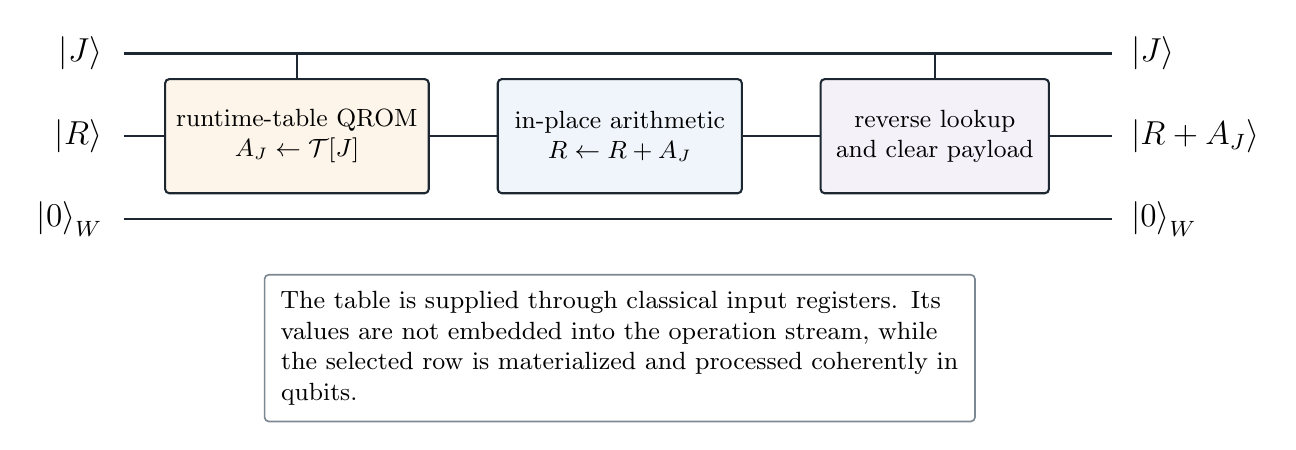
\begin{tikzpicture}[x=1cm,y=1cm]
  \node[anchor=east,font=\large] at (0,2.25) {$\ket{J}$};
  \node[anchor=east,font=\large] at (0,1.20) {$\ket{R}$};
  \node[anchor=east,font=\large] at (0,0.15) {$\ket{0}_{W}$};
  \draw[wire] (0.15,2.25) -- (12.7,2.25);
  \draw[wire] (0.15,1.20) -- (12.7,1.20);
  \draw[wire] (0.15,0.15) -- (12.7,0.15);
  \node[lookup,minimum width=2.6cm,minimum height=1.45cm] (load) at (2.35,1.20) {runtime-table QROM\\$A_J\leftarrow\mathcal T[J]$};
  \node[stage,minimum width=3.1cm,minimum height=1.45cm] (add) at (6.45,1.20) {in-place arithmetic\\$R\leftarrow R+A_J$};
  \node[replay,minimum width=2.9cm,minimum height=1.45cm] (unload) at (10.45,1.20) {reverse lookup\\and clear payload};
  \draw[wire] (2.35,2.25) -- (load.north);
  \draw[wire] (10.45,2.25) -- (unload.north);
  \node[anchor=west,font=\large] at (12.82,2.25) {$\ket{J}$};
  \node[anchor=west,font=\large] at (12.82,1.20) {$\ket{R+A_J}$};
  \node[anchor=west,font=\large] at (12.82,0.15) {$\ket{0}_{W}$};
  \node[note,text width=8.6cm,anchor=north] at (6.45,-0.55) {The table is supplied through classical input registers. Its values are not embedded into the operation stream, while the selected row is materialized and processed coherently in qubits.};
\end{tikzpicture}}
\caption{Runtime-table window interface implemented by the modified circuit.}
\label{fig:target-interface}
\end{figure}

The emitted register ABI is
\begin{equation}
(X,Y,J,\mathcal T_x[0],\mathcal T_y[0],\ldots,\mathcal T_x[2^w-1],\mathcal T_y[2^w-1]),
\label{eq:abi}
\end{equation}
where $X$ and $Y$ are 256-qubit coordinate registers, $J$ is a $w$-qubit quantum register, and every table coordinate is a 256-bit classical input register. The ABI requires $\mathcal T[0]=(0,0)$ as the classical encoding of $\mathcal O$. Thus, a $w=16$ instance exposes $2\cdot2^{16}$ coordinate registers. The operation stream refers to their bits through classical conditions; replacing one shifted $G$- or public-point table by another changes the input data rather than the circuit topology. The supplied evaluator populates these registers with the reference table $\mathcal T[j]=[j]G$, but the emitted circuit is not restricted to that table.

\section{Circuit-Level Modifications}

\subsection{Stage-local materialization}

The six-stage arithmetic order of \texttt{8e9c9a2} is retained. Only the boundaries at which the addend is consumed are changed. Stages~1 and~6 jointly load the two selected coordinates through one address traversal; Stage~3 loads only $x_J$. Every payload is removed before the dialog-GCD peaks.

\begin{figure}[ht]
\centering
\resizebox{\linewidth}{!}{%
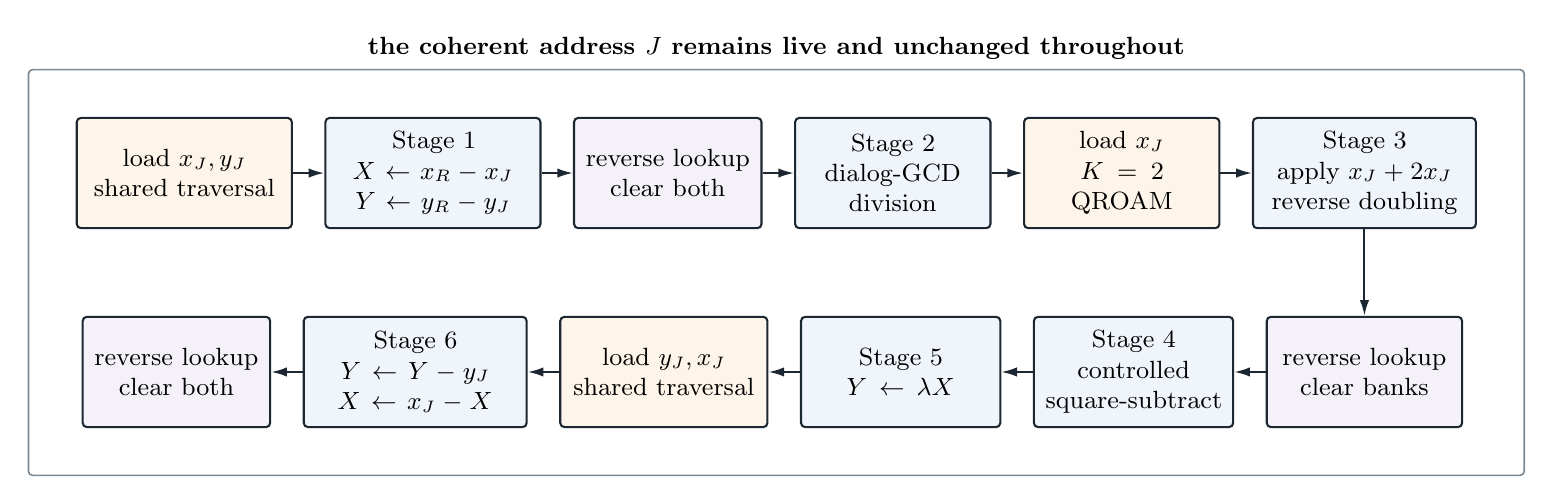
\begin{tikzpicture}[node distance=4mm and 4mm]
  \node[lookup,text width=2.45cm,minimum height=1.4cm] (lxy) {load $x_J,y_J$\\shared traversal};
  \node[stage,right=of lxy,text width=2.45cm,minimum height=1.4cm] (diff) {Stage 1\\$X\gets x_R-x_J$\\$Y\gets y_R-y_J$};
  \node[replay,right=of diff,text width=2.1cm,minimum height=1.4cm] (uxy) {reverse lookup\\clear both};
  \node[stage,right=of uxy,text width=2.2cm,minimum height=1.4cm] (div) {Stage 2\\dialog-GCD\\division};
  \node[lookup,right=of div,text width=2.2cm,minimum height=1.4cm] (lx) {load $x_J$\\$K=2$ QROAM};
  \node[stage,right=of lx,text width=2.55cm,minimum height=1.4cm] (add3x) {Stage 3\\apply $x_J+2x_J$\\reverse doubling};
  \draw[flow] (lxy)--(diff); \draw[flow] (diff)--(uxy); \draw[flow] (uxy)--(div); \draw[flow] (div)--(lx); \draw[flow] (lx)--(add3x);
  \node[replay,below=11mm of add3x,text width=2.2cm,minimum height=1.4cm] (ux) {reverse lookup\\clear banks};
  \node[stage,left=of ux,text width=2.25cm,minimum height=1.4cm] (sq) {Stage 4\\controlled\\square-subtract};
  \node[stage,left=of sq,text width=2.25cm,minimum height=1.4cm] (mul) {Stage 5\\$Y\gets\lambda X$};
  \node[lookup,left=of mul,text width=2.35cm,minimum height=1.4cm] (lrec) {load $y_J,x_J$\\shared traversal};
  \node[stage,left=of lrec,text width=2.55cm,minimum height=1.4cm] (rec) {Stage 6\\$Y\gets Y-y_J$\\$X\gets x_J-X$};
  \node[replay,left=of rec,text width=2.1cm,minimum height=1.4cm] (urec) {reverse lookup\\clear both};
  \draw[flow] (add3x)--(ux); \draw[flow] (ux)--(sq); \draw[flow] (sq)--(mul); \draw[flow] (mul)--(lrec); \draw[flow] (lrec)--(rec); \draw[flow] (rec)--(urec);
  \node[note,fill=none,fit=(lxy)(add3x)(ux)(urec),inner sep=6mm,label={[font=\small\bfseries]above:the coherent address $J$ remains live and unchanged throughout}] {};
\end{tikzpicture}}
\caption{Stage-local lookup/use/replay schedule. The selected point is never retained through the arithmetic peak.}
\label{fig:stage-schedule}
\end{figure}

Stage~3 does not require a derived $3x$ table. It loads $x_J$ into a 257-qubit temporary register, first accumulates $x_J$ into $X$, reversibly doubles the temporary value modulo $p$, accumulates $2x_J$, reverses the doubling, and unloads the original $x_J$. Therefore, the update is $X\gets X+3x_J\pmod p$, while the ABI contains only the two source-coordinate columns. Stage~6 likewise derives reverse subtraction from the loaded $x_J$: for a nonidentity row it applies modular negation to $X$ and then adds $x_J$, giving $x_J-X\pmod p$. No embedded $x_J+1$ column is required.

\subsection{Identity row and generic-affine domain}

Row $J=0$ represents the elliptic-curve identity $\mathcal O$ and, by the ABI above, supplies zero coordinate payloads. The circuit computes a coherent predicate $b=[J\neq0]$, uses $b$ to control the square-subtract in Stage~4 and modular negation in Stage~6, and uncomputes $b$ at the end. When $J=0$, Stages~1--3 leave $(X,Y)$ at $(x_R,y_Rx_R^{-1})$ after division; Stage~4 is disabled; Stage~5 reverses the division map and restores $Y=y_R$; and Stage~6 leaves $X=x_R$. Hence the complete branch returns $R+\mathcal O=R$ without measuring $J$. For a valid nonidentity \texttt{secp256k1} accumulator, $x_R\neq0$ automatically: an affine point with $x_R=0$ would require $y_R^2=7$, whereas $7$ is a quadratic nonresidue modulo $p$.

The exceptional affine cases $R=A_J$ and $R=-A_J$ remain outside the circuit domain. They make the denominator $x_R-x_J$ vanish and require point doubling or an explicit identity output. This is the same generic-affine restriction used by the source circuit and Schrottenloher's point-addition construction; it is distinct from the table's identity row, which the modified circuit now handles.

\subsection{Low-peak arithmetic}

The QROM payload is live only near its consumer, but it still competes locally with carry ancillas. The modification suppresses carry venting at loaded-data sites and compares only the 64 most significant bits during its low-peak modular additions. This comparison agrees with a full-width comparison whenever those prefixes differ, but it is not exact when the prefixes are equal and lower bits determine the ordering. It is therefore a distribution-dependent approximation rather than an all-input guarantee. No new classical mismatch attributable to this comparison was observed in the paired 100,000-input corpus, but that empirical result does not establish worst-case correctness. The global maximum remains the inverse-application fold after all QROM payloads have been cleared.

\section{Runtime QROM and Exact Replay}

\subsection{Why an XOR lookup loads a table word}

For one table column $c_j\in\{0,1\}^{256}$, QROM implements
\begin{equation}
L_c:\quad \ket{j}\ket{z}\longmapsto\ket{j}\ket{z\oplus c_j}.
\label{eq:xor-load}
\end{equation}
If the payload starts in $\ket{0}$, then $0\oplus c_j=c_j$, so $L_c\ket{j}\ket{0}=\ket{j}\ket{c_j}$. Operationally, a reversible address traversal constructs the predicate selecting row $j$ and applies a classically conditioned CNOT to each payload position whose runtime table bit is one. By linearity,
\begin{equation}
\sum_j\alpha_j\ket{j}\ket{0}\longmapsto\sum_j\alpha_j\ket{j}\ket{c_j},
\label{eq:coherent-load}
\end{equation}
so the payload becomes correlated with the coherent address. Here $c_j$ is one coordinate column, such as $x_j$ or $y_j$, not the complete point $A_j$.

\subsection{$K=2$ QROAM and payload width}

The single-column Stage~3 lookup uses two-row blocking. Write $j=2h+\ell$, where $h$ contains the high $w-1$ address bits and $\ell$ is the least significant bit. The high-address traversal loads adjacent rows into two 256-qubit banks, and controlled swaps select the requested row:
\begin{equation}
\ket{h,\ell}\ket{0}_{B_0}\ket{0}_{B_1}\longmapsto\ket{h,\ell}\ket{c_{2h}}_{B_0}\ket{c_{2h+1}}_{B_1}\longmapsto\ket{h,\ell}\ket{c_{2h+\ell}}_{B_0}\ket{c_{2h+1-\ell}}_{B_1}.
\label{eq:qroam2}
\end{equation}
Because $j=2h+\ell$, $c_{2h+\ell}=c_j$ is precisely the selected word. The notation does not mean that $c_{2h+\ell}$ is the complete table point: in Stage~3 it is the $x$-coordinate word $x_j$.

\begin{figure}[ht]
\centering
\resizebox{0.94\linewidth}{!}{%
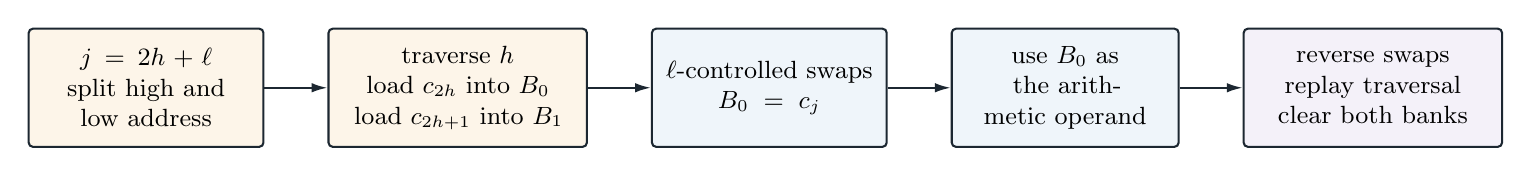
\begin{tikzpicture}[node distance=7mm and 8mm]
  \node[lookup,text width=2.7cm,minimum height=1.5cm] (split) {$j=2h+\ell$\\split high and low address};
  \node[lookup,right=of split,text width=3.0cm,minimum height=1.5cm] (pair) {traverse $h$\\load $c_{2h}$ into $B_0$\\load $c_{2h+1}$ into $B_1$};
  \node[stage,right=of pair,text width=2.7cm,minimum height=1.5cm] (swap) {$\ell$-controlled swaps\\$B_0=c_j$};
  \node[stage,right=of swap,text width=2.6cm,minimum height=1.5cm] (use) {use $B_0$ as\\the arithmetic operand};
  \node[replay,right=of use,text width=3.0cm,minimum height=1.5cm] (clean) {reverse swaps\\replay traversal\\clear both banks};
  \draw[flow] (split)--(pair); \draw[flow] (pair)--(swap); \draw[flow] (swap)--(use); \draw[flow] (use)--(clean);
\end{tikzpicture}}
\caption{$K=2$ QROAM used for the Stage~3 $x_J$ episode.}
\label{fig:qroam2}
\end{figure}

The construction does not store a 512-bit point in the 16 address qubits. Stages~1 and~6 temporarily allocate two 256-qubit payloads, and Stage~3 temporarily allocates the selected and adjacent 256-qubit banks shown in \eqref{eq:qroam2}. The width saving is temporal: these banks are cleared before the global dialog-GCD peak instead of remaining resident throughout the point addition. Consequently, their local 512-qubit storage increases the measured peak by only 11 qubits relative to the mixed-addition circuit.

\subsection{Exact replay unload}

After the arithmetic consumer preserves a loaded payload, applying the same XOR lookup again gives
\begin{equation}
L_c^2:\quad \ket{j}\ket{c_j}\longmapsto\ket{j}\ket{c_j\oplus c_j}=\ket{j}\ket{0}.
\label{eq:replay-unload}
\end{equation}
The reported circuit therefore reverses the $K=2$ swaps when applicable and replays the same runtime-table traversal. This exactly removes the payload without measuring it. The traversal's unary-routing AND ancillas are removed using measurement-based uncomputation with conditional phase correction. Under the QROM circuit identity, these corrections remove the phase introduced by routing cleanup, so the lookup/replay boundary leaves no row-dependent payload, ancilla, or address-dependent phase. The sparse phase failures reported for the complete point-addition circuit are end-to-end arithmetic failures and are not, by themselves, evidence of a residual QROM-selection phase. A measurement-based \emph{payload} unload remains implemented as an optional experiment, but the final resource and correctness results use payload replay.

\begin{table}[ht]
\centering
\small
\begin{tabular}{@{}lrrrl@{}}
\toprule
Episode & Load Toffoli & Replay Toffoli & Total & Runtime columns \\
\midrule
Coordinate differences & 65,534 & 65,534 & 131,068 & $x_J,y_J$ \\
Apply $3x_J$ ($K=2$) & 33,022 & 33,022 & 66,044 & $x_J$ \\
Output recovery & 65,534 & 65,534 & 131,068 & $y_J,x_J$ \\
\midrule
Total & 164,090 & 164,090 & 328,180 & six traversals \\
\bottomrule
\end{tabular}
\caption{Instrumented nonlinear QROM cost for $w=16$. The complete stream also contains 167,772,160 classically conditioned table-payload CNOTs across loading and replay.}
\label{tab:qrom-cost}
\end{table}

\section{Circuit-to-Source Correspondence}

\begin{table}[ht]
\centering
\footnotesize
\begin{tabularx}{\linewidth}{@{}>{\raggedright\arraybackslash}p{2.65cm}>{\raggedright\arraybackslash}p{6.15cm}X@{}}
\toprule
Circuit role & Principal source entry points & Effect \\
\midrule
Runtime ABI & \code{trailmix\_ludicrous/mod.rs}: \code{build\_trailmix\_ludicrous\_ops} & Declares $X,Y,J$ and the $2\cdot2^w$ classical coordinate registers; no table values are written into the emitted circuit. \\
Runtime payload controls & \code{qrom.rs}: \code{xor\_payload}, \code{load\_word}, \code{load\_two\_words}; \code{point\_add/mod.rs}: \code{cx\_if} & Emits CNOT operations whose classical condition is the corresponding runtime table bit. \\
Stages 1 and 6 & \code{ec\_add.rs}: \code{qrom\_coord\_differences}, \code{qrom\_coord\_recover} & Loads two coordinate columns through a shared traversal, applies the coordinate maps, and immediately replays the lookup. \\
Runtime $3x_J$ & \code{ec\_add.rs}: \code{qrom\_coord\_add3x} & Loads only $x_J$, applies $x_J+2x_J$, reverses the modular doubling, and unloads $x_J$. \\
Identity handling & \code{ec\_add.rs}: \code{toggle\_nonzero\_address}; \code{square.rs}: controlled square-subtract & Constructs $[J\neq0]$, controls the two operations that distinguish the identity branch, and uncomputes the predicate. \\
Exact unload & \code{qrom.rs}: \code{unload\_word}, \code{unload\_two\_words}, \code{emit\_qroam2\_replay\_unload} & Reverses swaps and replays the XOR lookup to clear payload and routing qubits exactly. \\
Peak-width control & \code{arith.rs}: low-peak modular add/subtract variants & Avoids simultaneous payload and wide carry-vent allocations and uses a 64-bit upper comparison at the three QROM-use sites. \\
Validation only & \code{eval\_circuit.rs}: shared-corpus generation, runtime-table initialization, paired baseline/window evaluation, durable checkpointing, and correlated sequence runner & Supplies arbitrary table values and verifies coordinates, address, incremental phase, and non-interface ancillas. These changes do not alter the emitted circuit. \\
\bottomrule
\end{tabularx}
\caption{Correspondence between circuit-level changes and implementation entry points.}
\label{tab:source-map}
\end{table}

These changes establish window compatibility because $J$ is a genuine quantum register, every table-dependent payload operation is controlled by the externally supplied table bits, arithmetic consumes qubit payloads, and exact replay removes all which-row information outside $J$. The resulting circuit topology can therefore be reused with the shifted tables $\mathcal T_G^{(i)}[j]=[j2^{iw}]G$ or $\mathcal T_P^{(i)}[j]=[j2^{iw}]P$ required by a complete windowed scalar multiplication.

\section{Resource Measurements}

The fully emitted $w=16$ circuit contains 213,387,745 operations. Its measured peak remains the inverse-application fold, where all QROM payloads have already been released. Table~\ref{tab:resources} compares the result with the reported \texttt{8e9c9a2} operating point. The two executed-Toffoli values are measured on their respective deterministic 9,024-input evaluator supports, so the table characterizes resource overhead rather than a paired error experiment. By contrast, the abstract, Table~\ref{tab:paired-100k-results}, and the conclusion report $T$ on the common 100,000-input corpus; small differences between the two sets of averages are expected because executed Toffoli cost is input-dependent.

\begin{table}[ht]
\centering
\small
\begin{tabular}{@{}lrrr@{}}
\toprule
Metric & Original \texttt{8e9c9a2} & Runtime-table $w=16$ & Change \\
\midrule
Peak logical width $Q$ & 1,151 & 1,162 & $+11$ ($+0.96\%$) \\
Average executed Toffoli $T$ & 1,299,453 & 1,684,156.770 & $+384,703.770$ ($+29.61\%$) \\
$Q\times T$ & 1,495,670,403 & 1,956,990,167 & $+30.84\%$ \\
Static emitted operations & 9,133,449 & 213,387,745 & $23.36\times$ \\
\bottomrule
\end{tabular}
\caption{Resource overhead of coherent runtime-table selection on the circuits' respective deterministic 9,024-input evaluator supports. Table-payload CNOTs dominate the static stream and are not counted as Toffoli gates.}
\label{tab:resources}
\end{table}

The final circuit uses one more qubit and more Toffoli work than the earlier fixed-table, measurement-unload prototype. That increase is the cost of closing the principal interface and cleanup gaps: table data are now runtime inputs, and every payload is removed by exact replay. The persistent $w=16$ address itself does not imply a 16-qubit increase in $Q$, because the original and modified circuits have different concurrent scratch allocations at their maxima. The $Q\times T$ comparison follows the challenge convention and therefore does not price the 167,772,160 emitted table-payload CNOTs, measurements, classical feed-forward, or table storage. The $23.36\times$ increase in static operations may be material under a fault-tolerant architecture that assigns non-negligible cost to these operations. This note compares the adapter only with its \texttt{8e9c9a2} baseline and makes no cross-work dominance claim.

\section{Validation}

\subsection{Full 16-bit evaluation}

The final 16-bit circuit was evaluated on 9,024 deterministic pseudorandom cases. Each case supplies the complete runtime table $\mathcal T[j]=[j]G$, samples a target accumulator and coherent address, and classically computes the expected generic-affine sum. Cases with nonzero $J$ and $x_R=x_J$ are excluded because they fall outside the declared generic-affine domain; $J=0$ is retained.

\begin{table}[ht]
\centering
\small
\begin{tabular}{@{}lr@{}}
\toprule
Outcome & Count \\
\midrule
Classical mismatches & 14 / 9,024 ($0.1551\%$) \\
Phase-failure shots & 10 / 9,024 ($0.1108\%$) \\
Ancilla-failure shots & 0 / 9,024 ($0\%$) \\
Shots failing any channel & 20 / 9,024 ($0.2216\%$) \\
Identity selections & 1 / 9,024 ($0.0111\%$) \\
\bottomrule
\end{tabular}
\caption{Validation of the final $w=16$ runtime-table circuit. Failure categories overlap.}
\label{tab:full-errors}
\end{table}

The identity case returned the input coordinates, preserved $J=0$, and had no classical, phase, or ancilla failure. Exact payload replay produced no dirty payload or routing ancilla on any shot. The residual classical and phase failures occur on ordinary inputs within the declared generic-affine domain and are distinct from the excluded cases $R=\pm A_J$. They are consistent with the fixed-length dialog-GCD schedule and inherited finite-width arithmetic; the 64-bit upper comparison is an additional potential approximation, although the experiment does not isolate any failure caused by it. The circuit does not supply a coherent flag for any of these arithmetic failures.

The evaluator records one durable row per input and one commit record per 64-shot batch. On restart, it truncates any uncommitted input tail, reconstructs aggregate counts, and evaluates only unfinished batches. This checkpoint mechanism produced the complete 9,024-case ledger used above.

\subsection{Paired 100,000-input random-corpus comparison}

To compare the arithmetic error of the two interfaces without allowing either operation stream to select its own test set, we generated 100,000 cases from the explicit seed \code{ecdsafail-windowed-independent-random-100k-v1}. This seed is independent of both circuit hashes and therefore does not use the benchmark's Fiat--Shamir sampling rule. Each case contains a random nonidentity accumulator $R=[a]G$, a uniformly sampled 16-bit address $j$, the addend $A_j=[j]G$, and the expected result $R+A_j$. Cases with $R=\pm A_j$ are resampled because they lie outside the common generic-affine domain, whereas $j=0$ is retained as the identity row. Joining the two input ledgers by index found no mismatch in their address, accumulator, addend, or expected-output columns.

\begin{table}[ht]
\centering
\small
\begin{tabular}{@{}lrr@{}}
\toprule
Metric & Original \texttt{8e9c9a2} & Runtime-table $w=16$ \\
\midrule
Peak logical width $Q$ & 1,151 & 1,162 \\
Average executed Toffoli $T$ & 1,299,440.793 & 1,684,160.924 \\
$Q\times T$ & 1,495,656,352.743 & 1,956,994,993.688 \\
Classical-output failures & 154 ($0.1540\%$) & 151 ($0.1510\%$) \\
Phase failures & 115 ($0.1150\%$) & 117 ($0.1170\%$) \\
Ancilla failures & 0 & 0 \\
Inputs failing any channel & 192 ($0.1920\%$) & 191 ($0.1910\%$) \\
Wilson 95\% interval, any channel & $[0.1667\%,0.2211\%]$ & $[0.1658\%,0.2200\%]$ \\
\bottomrule
\end{tabular}
\caption{Paired evaluation on 100,000 independently seeded inputs. Failure categories overlap.}
\label{tab:paired-100k-results}
\end{table}

Of the 100,000 inputs, 162 fail at least one channel in both circuits, 30 fail only in the baseline, 29 fail only in the windowed circuit, and 99,779 fail in neither. A two-sided exact sign test on the 59 discordant outcomes gives $p_{\mathrm{sign}}=1.0$. All 151 classical-output failures of the windowed circuit are also classical failures of the baseline; the windowed circuit introduces no new classical mismatch on this corpus and removes three, including both sampled identity rows. The sets of phase-failing inputs differ because the two operation streams and their measurement histories are not identical, but this end-to-end experiment does not attribute a phase failure to a particular subroutine. The observed one-input difference in total failures is negligible relative to sampling uncertainty, so the experiment supports comparable empirical error rates rather than an accuracy advantage for either circuit.

On this shared corpus, coherent runtime-table selection adds 11 logical qubits ($0.956\%$), 384,720.131 average executed Toffoli gates ($29.607\%$), and $30.845\%$ to the $Q\times T$ proxy. The evaluator writes one input record before committing each 64-input batch, synchronizes both files to durable storage, and binds each checkpoint to the interface, seed, requested corpus size, resource dimensions, and operation-stream fingerprint. A restarted run truncates any uncommitted input tail and skips every committed batch, allowing the experiment to resume without discarding completed cases.

\subsection{Correlated multi-call tests for \texorpdfstring{$w=0,\ldots,5$}{w=0,...,5}}

To test composition rather than isolated calls, the evaluator retains one accumulator, supplies a new coherent address, applies the same emitted kernel four times, and checks the intermediate accumulator, preserved address, phase increment, and every non-interface qubit after each call. For each $w\in\{0,\ldots,5\}$, 256 four-call sequences were evaluated, giving 1,024 additions per width and 6,144 calls in total.

\begin{table}[ht]
\centering
\small
\begin{tabular}{@{}rrrrr@{}}
\toprule
$w$ & Identity selections & Any-failure sequences & Ancilla failures & Per-call average $T$ \\
\midrule
0 & 1,024 / 1,024 & 0 / 256 & 0 & 1,312,343.476 \\
1 & 473 / 1,024 & 2 / 256 & 0 & 1,321,065.429 \\
2 & 253 / 1,024 & 0 / 256 & 0 & 1,322,636.318 \\
3 & 125 / 1,024 & 4 / 256 & 0 & 1,324,426.755 \\
4 & 63 / 1,024 & 0 / 256 & 0 & 1,326,497.064 \\
5 & 30 / 1,024 & 1 / 256 & 0 & 1,328,558.680 \\
\bottomrule
\end{tabular}
\caption{Correlated four-call tests. The sparse classical/phase failures reflect the inherited approximate arithmetic; no sequence leaves QROM or arithmetic ancillas live.}
\label{tab:small-window-tests}
\end{table}

The $w=0$ circuit consists entirely of identity selections and is exact on this corpus. The $w=1$ emitter and unload path also complete normally, closing the earlier base-case crash. Most importantly, the previous failure rate proportional to $2^{-w}$ disappears: row zero is no longer treated as the affine point $(0,0)$.

\section{Reproduction}

The implementation is maintained on branch \href{https://github.com/jieyilong/ecdsafail-challenge/tree/codex/windowed-8e9c9a2}{\code{codex/windowed-8e9c9a2}} of \code{jieyilong/ecdsafail-challenge}. From its worktree:
\begin{lstlisting}
cargo build --release --locked --offline \
  --bin build_circuit --bin eval_circuit

WINDOWED_MODE=1 WINDOW_BITS=16 SINGLE_CCX_FANOUT_DISABLE=1 \
  ./target/release/build_circuit

WINDOWED_MODE=1 WINDOW_BITS=16 WINDOWED_TESTS=9024 \
  WINDOWED_MAX_ERROR_RATE=1 EVAL_THREADS=8 \
  EVAL_CHECKPOINT_DIR=<checkpoint-dir> \
  ./target/release/eval_circuit \
  --note runtime-table-k16-replay-unload
\end{lstlisting}
Set \nolinkurl{WINDOWED_SEQUENCE_CALLS=4} to select the correlated test mode; repeat emission and evaluation with \nolinkurl{WINDOW_BITS=0}, \ldots, \code{5} to reproduce Table~\ref{tab:small-window-tests}.

\newpage
The paired 100,000-input experiment uses the same explicit seed and separate checkpoint directories for the two interfaces:
\begin{lstlisting}
EVAL_SHARED_SEED=ecdsafail-windowed-independent-random-100k-v1 \
  MIXED_WINDOW_BITS=16 EVAL_TESTS=100000 EVAL_THREADS=8 \
  EVAL_MAX_ERROR_RATE=1 EVAL_CHECKPOINT_DIR=<baseline-dir> \
  ecdsafail run

EVAL_SHARED_SEED=ecdsafail-windowed-independent-random-100k-v1 \
  WINDOWED_MODE=1 WINDOW_BITS=16 SINGLE_CCX_FANOUT_DISABLE=1 \
  WINDOWED_TESTS=100000 WINDOWED_MAX_ERROR_RATE=1 EVAL_THREADS=8 \
  EVAL_CHECKPOINT_DIR=<windowed-dir> ecdsafail run
\end{lstlisting}
Reissuing either command validates the checkpoint manifest and resumes only unfinished batches. The compact totals accompanying this note are in \code{paired\_100k\_counts.tsv}.

\section{Limitations}

\begin{itemize}
\item \textbf{Generic-affine exceptional cases.} The identity table row is supported, but $R=A_J$ and $R=-A_J$ remain outside the circuit domain, as in the underlying generic-affine construction.
\item \textbf{Approximate arithmetic on ordinary inputs.} Independently of the exceptional cases above, the inherited fixed-length dialog-GCD and finite-width arithmetic produce sparse classical and phase errors on generic-affine inputs. The window-specific 64-bit comparison introduces a further worst-case approximation, although it produced no identifiable new classical mismatch on the paired corpus. The modified circuit does not convert any arithmetic failure into a coherent flag.
\item \textbf{Finite-support and composition.} The experiments establish behavior only on the stated corpora; they are not an all-input proof or a coherent full-attack error estimate. In a complete Shor computation, silent errors can accumulate coherently across repeated additions and cannot be interpreted as independently retryable classical failures without an additional error model or detection mechanism.
\item \textbf{Kernel rather than full Shor.} The branch implements a reusable runtime-table point-addition call. A complete attack must instantiate all shifted $G$ and $P$ tables, schedule all windows, and validate the complete double-scalar multiplication and Fourier/postprocessing layers.
\item \textbf{Accounting convention.} Resource counts follow the challenge model, which optimizes logical qubits times average executed Toffoli gates. The emitted table-payload CNOTs dominate the $23.36\times$ larger static operation stream but do not contribute to $T$; a fault-tolerant architecture may assign non-negligible costs to these Clifford operations, classical table storage, measurements, and feed-forward.
\end{itemize}

\section{Conclusion}

The revised construction closes the principal lookup-interface gaps of the fixed-table prototype. It exposes the complete classical point-table ABI, conditions QROM on runtime table bits, derives temporary values within the circuit, handles the identity row, supports $w=0$ and $w=1$, and exactly clears every payload by replay. The resulting 16-bit kernel stays within the requested width bound at $Q=1{,}162$. On the independently seeded 100,000-input corpus, it uses $T=1{,}684{,}160.924$ average executed Toffoli gates and has a $0.1910\%$ any-channel error rate, statistically indistinguishable from the baseline's $0.1920\%$ rate in the paired comparison. These figures follow the challenge's $Q\times T$ accounting; the static operation stream is $23.36\times$ larger and may matter under other architectures. The result is therefore a window-compatible kernel under the stated benchmark interface, not a lower-cost competition submission or a validated full-Shor circuit. Its remaining limitations are approximate arithmetic without a coherent failure flag, finite-support validation, the standard generic-affine exceptional cases, and the absence of full-Shor integration.

\end{document}
